\textbf{Direction Fields and Euler's method}
\begin{figure}[h]
    \centering
    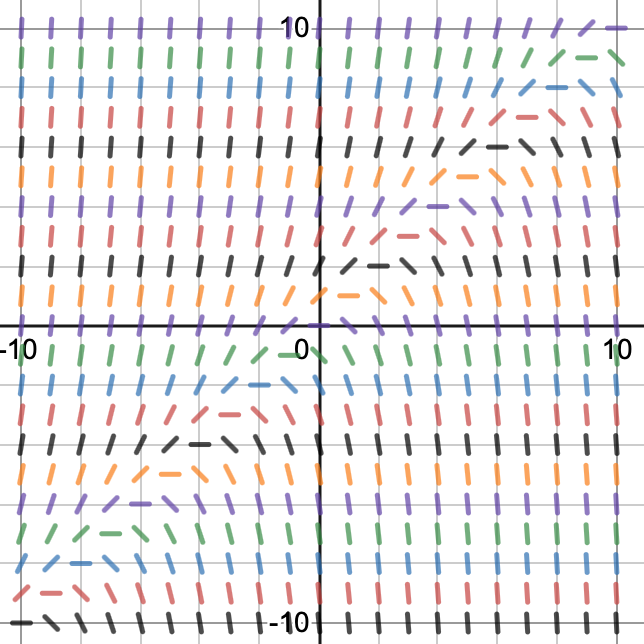
\includegraphics[scale=0.30]{1.png}
    \label{fig:1}
\end{figure}
\begin{align}
   y'=y-x
\end{align}
\begin{figure}[h]
    \centering
    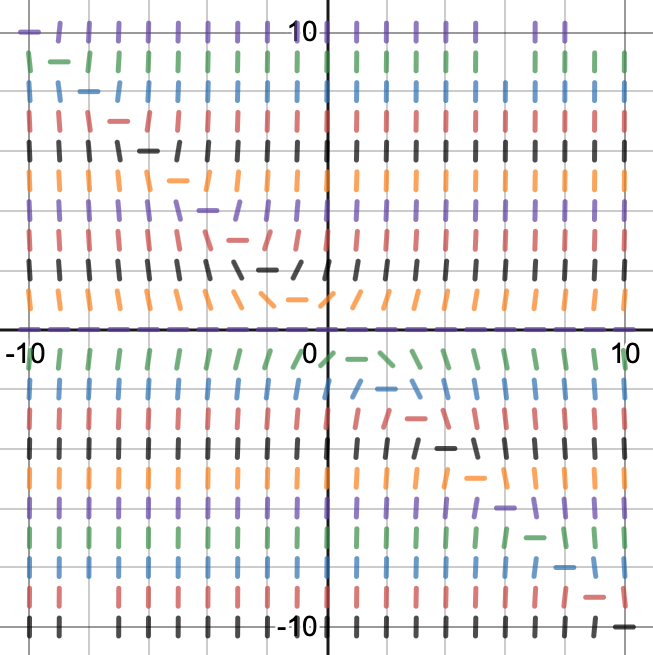
\includegraphics[scale=0.30]{2.png}
    \label{fig:2}
\end{figure}
\begin{align}
   y'=xy+y^{2}
\end{align}

